\documentclass[12pt]{article}
\usepackage[utf8]{inputenc}
\usepackage[a4paper,top=3cm,bottom=2cm,left=2.5cm,right=2.5cm,marginparwidth=3cm]{geometry}
\usepackage{biblatex}
\usepackage{appendix}
\usepackage{graphicx}
\usepackage{caption}
\usepackage{subcaption}
\usepackage{float}
\usepackage{hyperref}
\addbibresource{references.bib}

\title{\vspace{-3cm}Forecasting Trade Balance in Goods and Services\\ for the United States}
\bigskip
\bigskip
\bigskip
\author{
  \textbf{Agam Goyal}\\
  \texttt{agoyal25@wisc.edu}
  \and
  \textbf{Malkom Castellanos}\\
  \texttt{mcastellano3@wisc.edu}
}
\bigskip
\bigskip
\bigskip
\date{May 3, 2022}

\begin{document}

\maketitle

\section{Introduction}

The economic variable that we chose to forecast is the U.S. International Trade Balance in Goods and Services. International Trade Balance in Goods and Services attempts to accurately measure the trade balance of the United States, which is the difference between imports and exports measured in the millions of US dollars (\$).\\

This economic time series also captures what the top exports and imports in the United States were in a given month. However, for the purpose of the forecast, we will be looking at the value of the Trade Balance for the coming 12 months. To provide a more complete picture of the forecasts, we look at both point and interval forecasts.

\section{Data and Metrics}

The original publisher of the data we use is the Bureau of Economic Analysis (BEA). However, we obtained the data from the Federal Reserve Economic Data (FRED)\cite{data} using the FRED code \texttt{BOPGSTB}.\\

For the purpose of comparing different models we use for our data, the metric we use is the Akaike Information Criterion (AIC) to choose the best forecasting model. Since we are just beginning to work out a model for the Trade Balance time series, we believe that all models we come up with are just approximations of the true model, and our goal here is to find the best approximation, rather than finding the true model\cite{aic}. Moreover, we do not have access to out-of-sample data. These are the reasons for us to choose the AIC criterion over others like the Bayesian Information Criterion (BIC).

\section{Methods and Models\footnote{All code used to generate the results presented in the paper as well as the plots in the appendix can be found on \url{https://github.com/AGoyal0512/forecasting_project}}}

To begin exploring the nature of the time series data, we look at the auto-correlation function and the partial auto-correlation function and plot correlograms for the same. We see that the auto-correlation correlogram shows a slow decay trend and the partial auto-correlation correlogram seems to show no fixed trend (see \texttt{Appendix A}), except for indicating 7 significant lags after which the subsequent lags become insignificant. These trends suggest that we should look at an Autoregressive (AR) model for our forecast\cite{ar}.\\

Since the partial auto-correlation correlogram shows us that the first 7 lags would be important to look at for our AR model, we went ahead and ran the \texttt{ARIMA(7, 0, 0)} model on the time series data. On doing so, we saw that only the \texttt{p-values} for the first 4 lags were significant, and the AIC for this model was \texttt{6838.614} (See \texttt{Appendix B}). Updating the forecast model to just an autoregressive model of order 4 or \texttt{ARIMA(4, 0, 0)}, we got that all the four lags are significant, and more importantly, our AIC value was also lower at \texttt{6835.714}, which was the motivating factor for us to move forward with this model.\\

Before proceeding, we wanted to check for stationarity in our model, and see if we need any fixes to make the series stationary if it is non-stationary. For this, we used the Augmented Dickey-Fuller (ADF) test\cite{stationarity}. In this test, our null-hypothesis was that of assuming non-stationarity in the time series, while the alternative was the opposite, assuming stationary. We decided to use a \texttt{0.05} size-of-test for this hypothesis test.\\

When we ran the ADF test on our original time series, we got a \texttt{p-value} of \texttt{0.922304}, which means that we clearly fail to reject the null hypothesis for non-stationarity, which implies that there is a good chance that our series possesses non-stationarity, and that our series has a unit root. To fix this, we decided to use the method of differencing, and took a one-differenced time series of our original data, and then re-ran the ADF test on this series (See \texttt{Appendix C}). This time we obtained a \texttt{p-value} of almost \texttt{0.000}, which indicates that we have a strong evidence to reject the null hypothesis and conclude that this new series is stationary. So we now decided to integrate the one-differenced component in our ARIMA model, to get the \texttt{ARIMA(4, 1, 0)}. The lower AIC value of \texttt{6807.724} confirmed that we were thinking in the right direction (See \texttt{Appendix D}).\\

Laslty, we saw that on running the \texttt{ARIMA(4, 1, 0)} model, the $4^\text{th}$ lag became insignificant with a \texttt{p-value} of greater than \texttt{0.05}. So we decided to drop that lag and settle on an \texttt{ARIMA(3, 1, 0)} model, which had roughly a similar AIC value, but a lower BIC value\footnote{The reason we used BIC here is just for it to act as a sort of a tie-breaker, since the AIC values are very similar for being able to draw conclusions}, which was an indication that this model might be closer to what the true forecasting model for this time series looks like. See \texttt{Appendix D} for a detailed description of the model and its parameter estimates. 

\section{Forecasts and Discussions}

Having settled on the \texttt{ARIMA(3, 1, 0)} model, our next step was to check if the model actually works well on the data and whether it would be suitable for our out-of-sample forecasts. For this, we decided to split our time series into a testing set and a training set with a \texttt{2:1 train-test split}. We trained our model on the training set, and then used this model to predict values of the in-sample dates in the testing set.\\

On performing predictions on the test dataset, our Root Mean Squared Error\cite{rmse} was \texttt{3851.806}, which is a very reasonable error given that our observations are in the order of tens of thousands to almost a hundred thousand. Moreover, on plotting our predictions on top of the test data, we see that the forecast model performs a good job (See \texttt{Appendix F}).\\

Our first out-of-sample point forecast for the month of March is a trade balance in goods and services of \texttt{-\$ 89756.094707 million} for the United States. 

The point forecasts for the one upcoming year out-of-sample, for each of the 12 months lie at a trade balance in goods and services of \texttt{-\$ 89756.094707 million, -\$ 89427.186116 million, -\$ 91032.214411 million, -\$ 90702.505979 million, -\$ 90600.974737 million, -\$ 90999.122135 million, -\$ 90820.712238 million, -\$ 90819.462587 million, -\$ 90918.924467 million, -\$ 90851.954543 million, -\$ 90863.320926 million, and -\$ -90886.540965 million}.\\

The \texttt{95\%} interval forecasts along with the point forecasts for the 12 months are reported in a table in \texttt{Appendix E}. The plots showing these forecasts  with an overall plot of a part of the original time series with the 12 out-of-sample predictions can also be found in \texttt{Appendix F}. All observations are in the units of millions of United States \$.


\begin{center}
        \printbibliography
\end{center}

\pagebreak

\begin{center}
        \textbf{\Large\appendixname{ A}}
\end{center}

\begin{figure}[H]
	\centering
	\begin{subfigure}{1.0\textwidth}
		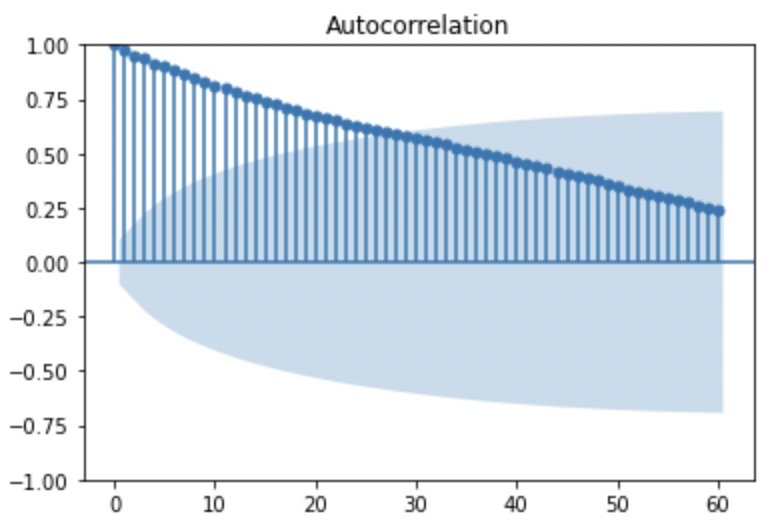
\includegraphics[width=\textwidth]{images/acf.png}
		\caption{Autocorrelation Correlogram}
	\end{subfigure}

	\begin{subfigure}{1.0\textwidth}
		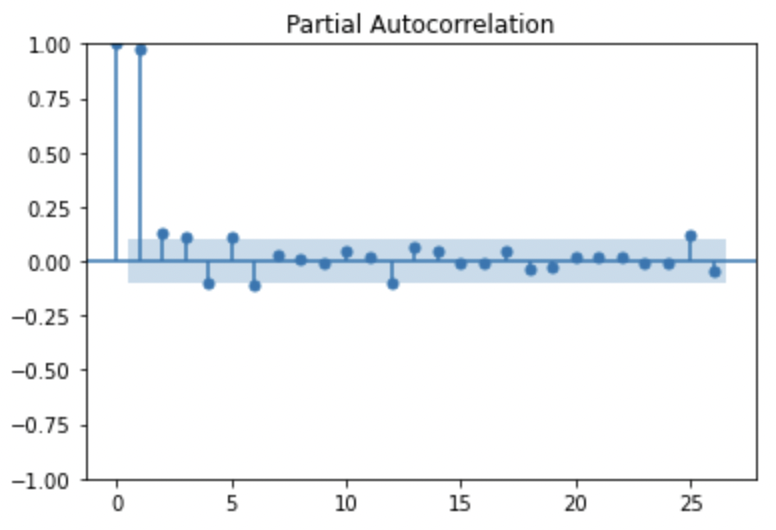
\includegraphics[width=\textwidth]{images/pacf.png}
		\caption{Partial Autocorrelation Correlogram}
	\end{subfigure}
\end{figure}

\begin{center}
        \textbf{\Large\appendixname{ B}}
\end{center}

\begin{figure}[H]
	\centering
	\begin{subfigure}{1.0\textwidth}
		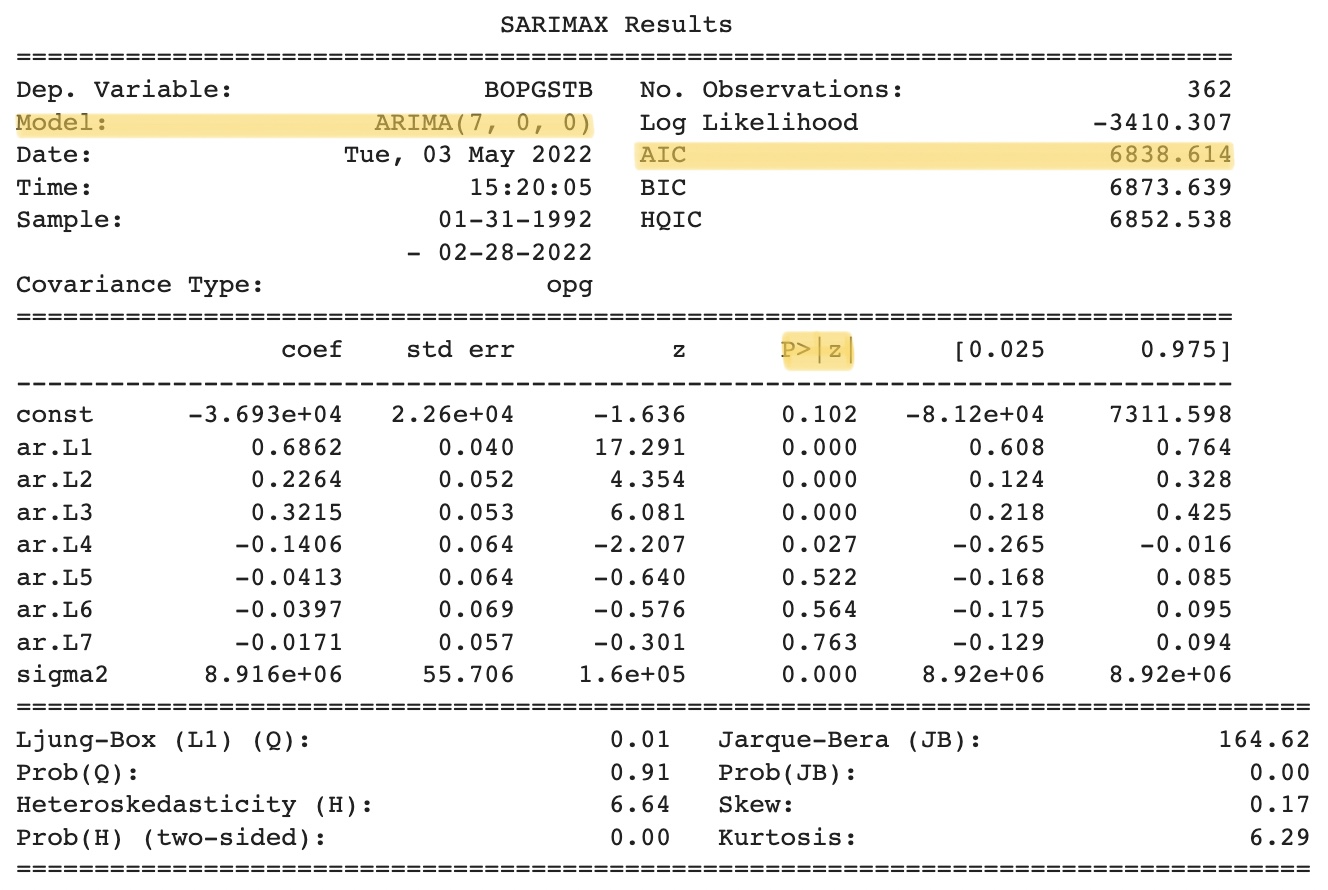
\includegraphics[width=\textwidth]{images/arima700.png}
		\caption{ARIMA(7, 0, 0) model}
	\end{subfigure}

    \bigskip
    
	\begin{subfigure}{1.0\textwidth}
		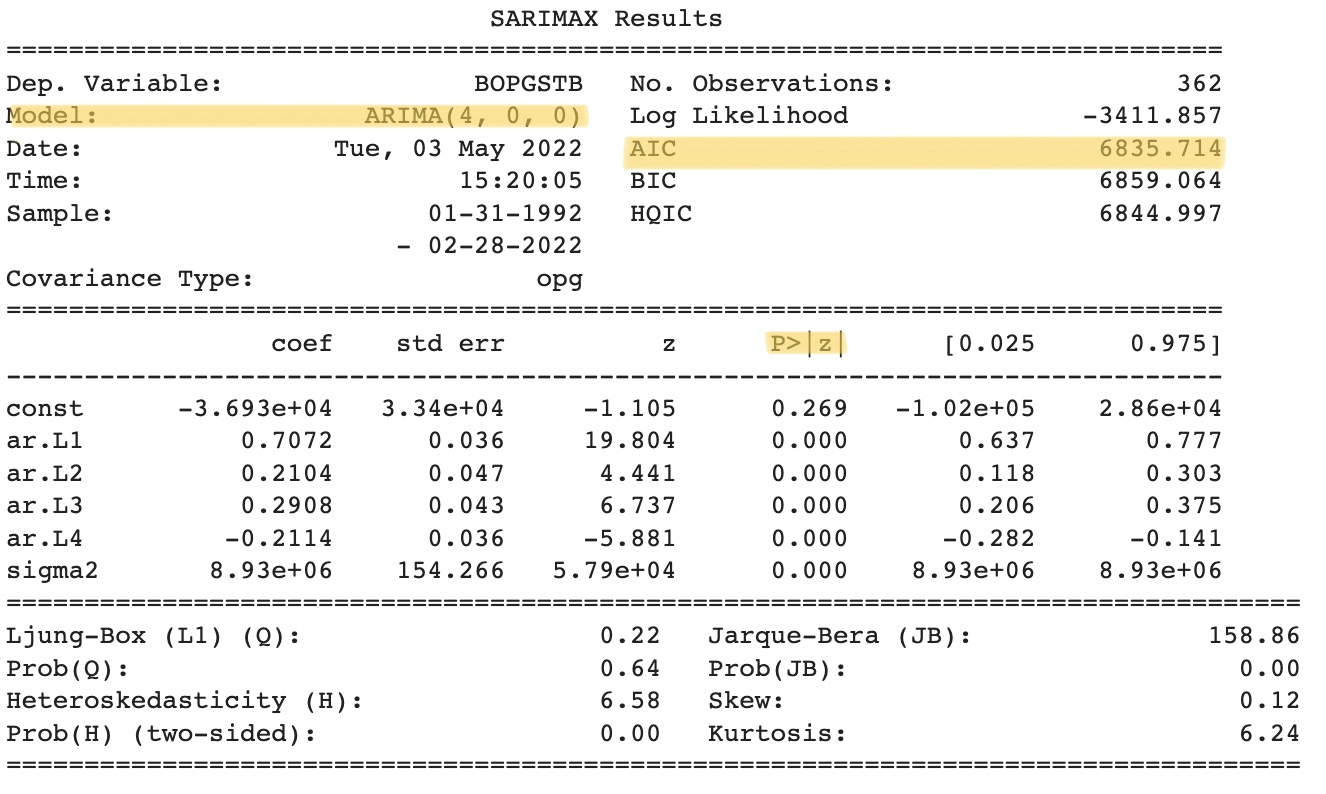
\includegraphics[width=\textwidth]{images/arima400.png}
		\caption{ARIMA(4, 0, 0) model}
	\end{subfigure}
\end{figure}

\pagebreak

\begin{center}
        \textbf{\Large\appendixname{ C}}
\end{center}

\begin{figure}[H]
	\centering
	\begin{subfigure}{1.0\textwidth}
		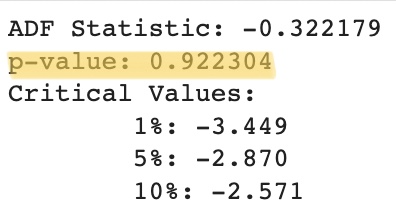
\includegraphics[width=\textwidth]{images/adf_pre.png}
		\caption{Results of the Augmented Dickey-Fuller Test BEFORE Differencing}
	\end{subfigure}

    \bigskip

	\begin{subfigure}{1.0\textwidth}
		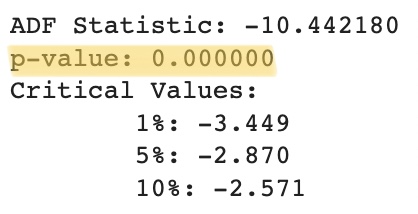
\includegraphics[width=\textwidth]{images/adf_post.png}
		\caption{Results of the Augmented Dickey-Fuller Test AFTER Differencing}
	\end{subfigure}
\end{figure}

\pagebreak

\begin{center}
        \textbf{\Large\appendixname{ D}}
\end{center}

\begin{figure}[H]
	\centering
	\begin{subfigure}{1.0\textwidth}
		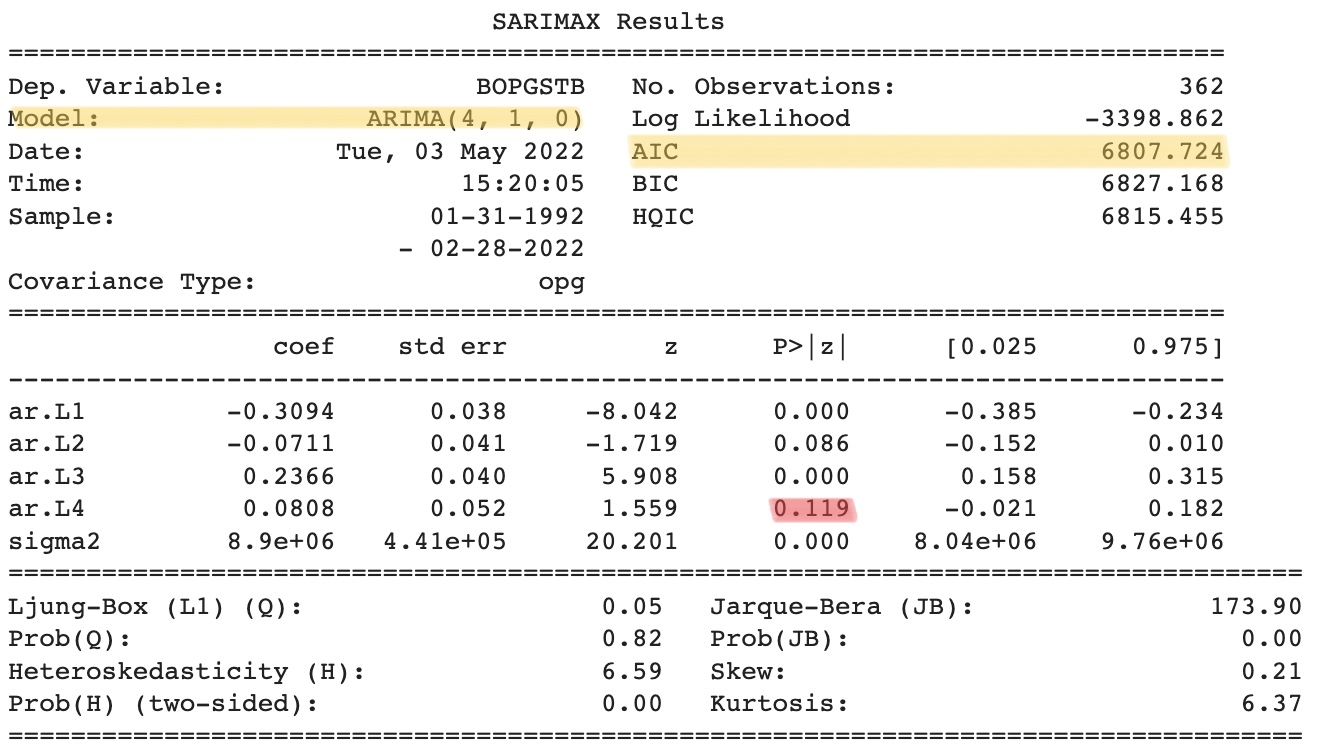
\includegraphics[width=\textwidth]{images/arima410.png}
		\caption{ARIMA(4, 1, 0) model}
	\end{subfigure}

    \bigskip

	\begin{subfigure}{1.0\textwidth}
		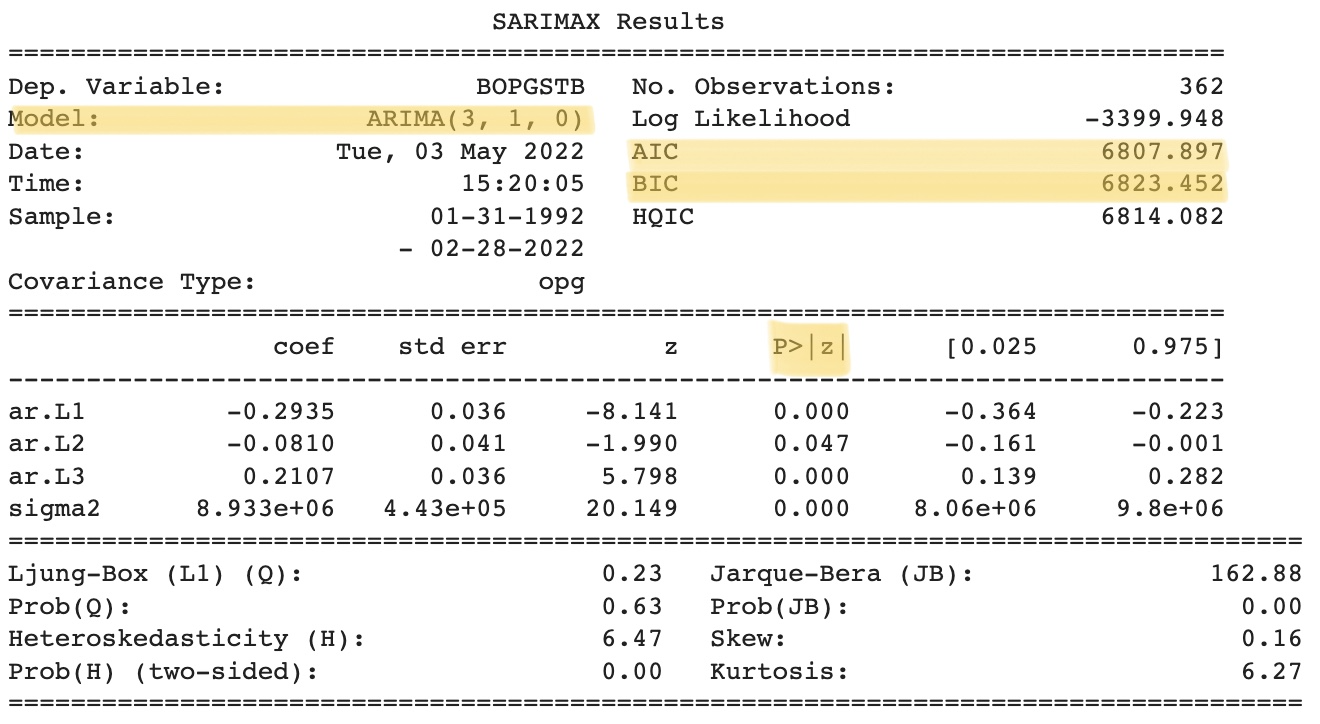
\includegraphics[width=\textwidth]{images/arima310.png}
		\caption{ARIMA(3, 1, 0) model}
	\end{subfigure}
\end{figure}

\pagebreak

\begin{center}
        \textbf{\Large\appendixname{ E}}
\end{center}

\begin{figure}[H]
	\centering
	\begin{subfigure}{1.0\textwidth}
		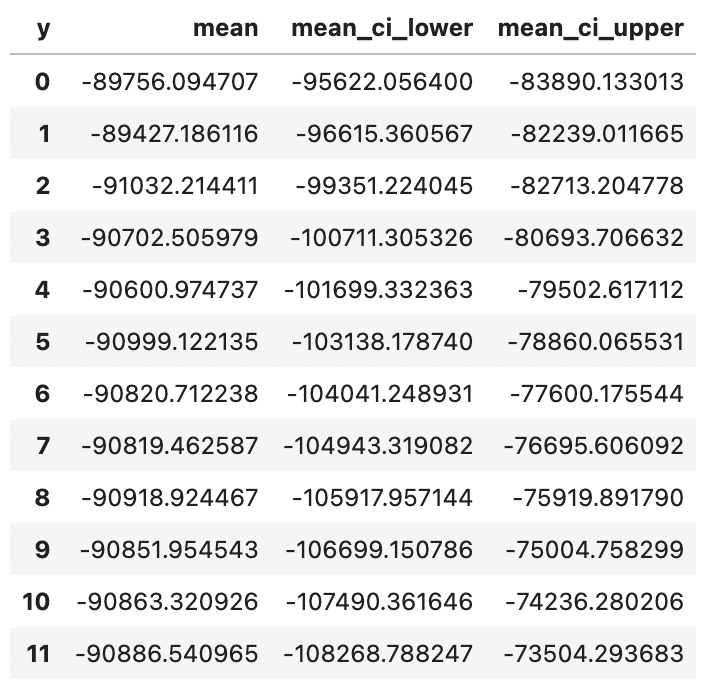
\includegraphics[width=\textwidth]{images/table.png}
		\caption*{Table containing Point and Interval Forecasts for 12 months}
	\end{subfigure}
\end{figure}

\pagebreak

\begin{center}
        \textbf{\Large\appendixname{ F}}
\end{center}

\begin{figure}[H]
	\centering
	\begin{subfigure}{0.6\textwidth}
		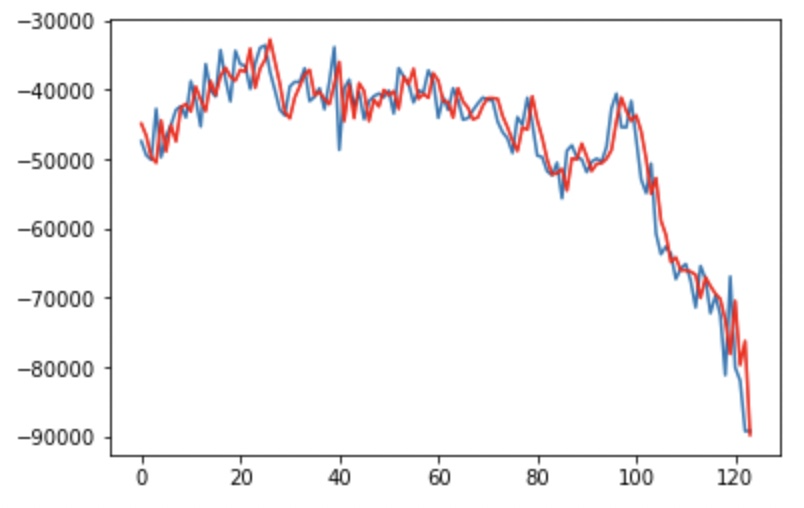
\includegraphics[width=\textwidth]{images/fit.png}
		\caption{Model Predictions (Red) with Testing Data (Blue)}
	\end{subfigure}

	\begin{subfigure}{0.6\textwidth}
		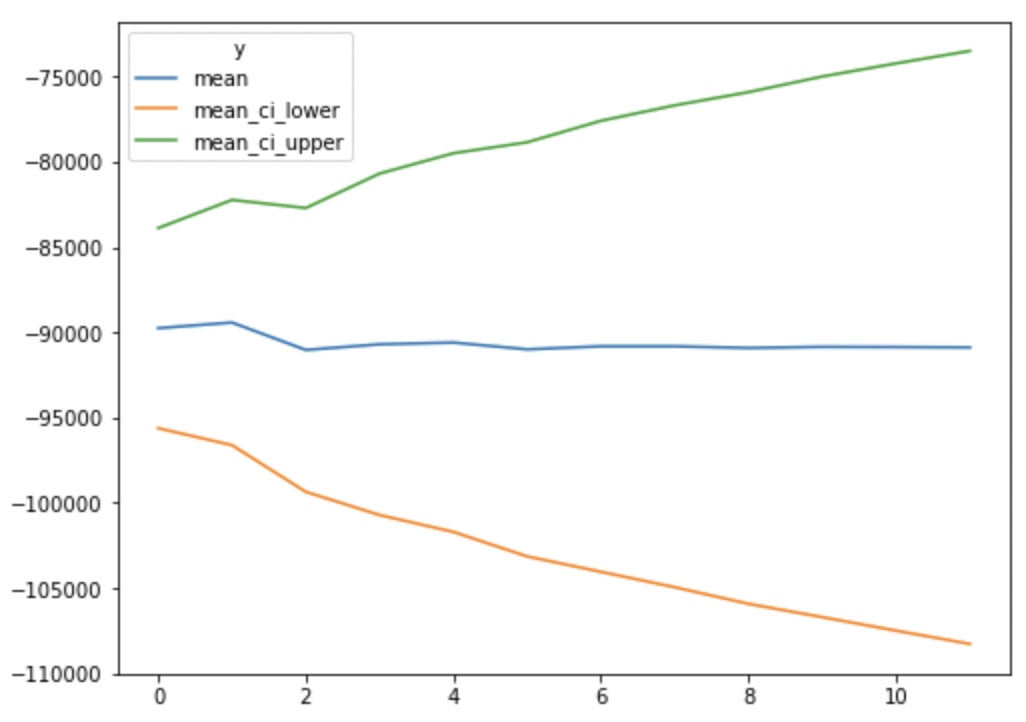
\includegraphics[width=\textwidth]{images/ci.png}
		\caption{Plot of Point and Interval Forecasts for 12 months}
	\end{subfigure}
	
	\begin{subfigure}{0.6\textwidth}
		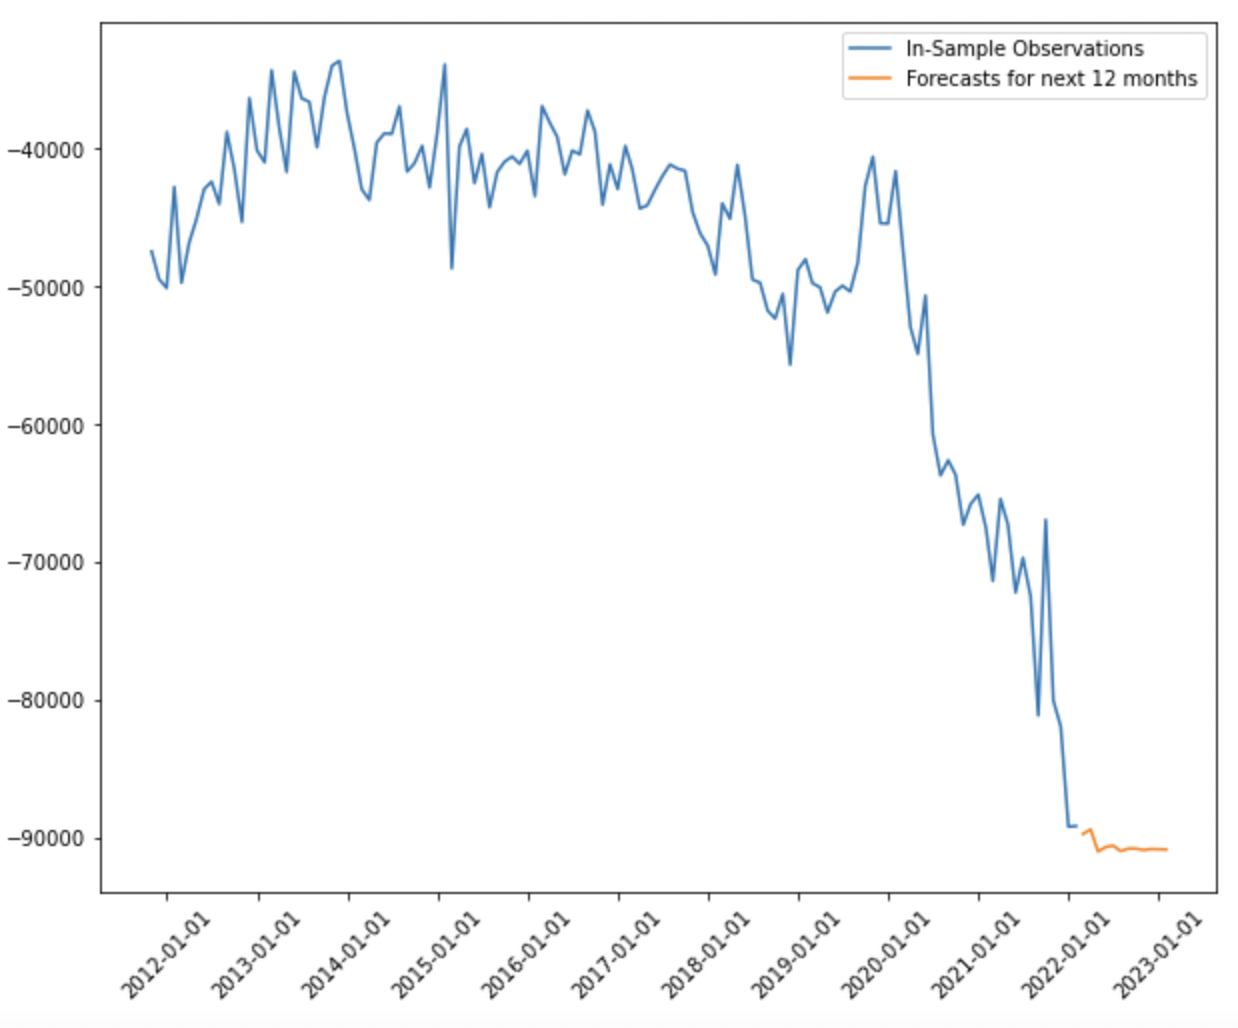
\includegraphics[width=\textwidth]{images/plot.png}
		\caption{Overall plot for Last 12 Years with Forecasts}
	\end{subfigure}
\end{figure}

\end{document}
